\documentclass{standalone}
\usepackage{tikz}
\usetikzlibrary{arrows}
\usepackage{fontspec}
    \setmainfont{Charis SIL}
\begin{document}
% In the preamble:

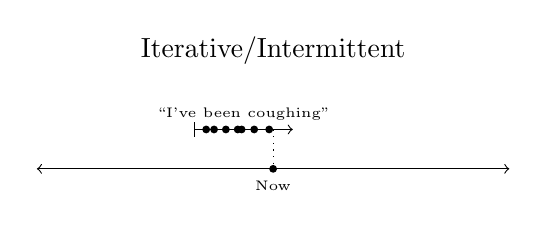
\begin{tikzpicture}[label distance=5mm]
    \draw [-, dotted] (0,0.5) node [] {} -- (-0,0) node[midway,above,sloped] (TextNode) {\tiny };
  \draw [<-, solid] (-3,0) node [] {} -- (-0.45,0) node[midway,above,sloped] (TextNode) {\tiny };
  \draw [-, solid] (-0.45,0) node [] {} -- (0.45,0) node[midway,above,sloped] (TextNode) {\tiny };
  \draw [->, solid] (0.45,0) node [] {} -- (3,0) node[midway,above,sloped] (TextNode) {\tiny };
  \draw [|->, solid ] (-1,0.5) node [] {} -- (0.25,0.5) node[midway,above] (TextNode) {\tiny ``I've been coughing''};
      \draw (-0.75,0.5) node[circle,fill,inner sep=1pt]{};
      \draw (-0.4,0.5) node[circle,fill,inner sep=1pt]{};
      \draw (-0.24,0.5) node[circle,fill,inner sep=1pt]{};
      \draw (-0.05,0.5) node[circle,fill,inner sep=1pt]{};
      \draw (-0.45,0.5) node[circle,fill,inner sep=1pt]{};
      \draw (-0.6,0.5) node[circle,fill,inner sep=1pt]{}; 
      \draw (-0.85,0.5) node[circle,fill,inner sep=1pt]{}; 

      \draw (0,-0) node[circle,fill,inner sep=1pt]{};

 \draw (0,-0.4) node[anchor=south]{\tiny Now};

 \draw (0,1.2) node[anchor=south]{Iterative/Intermittent};

\end{tikzpicture}

\end{document}
